\section{Model}
\label{sec:model}

We model Large Language Model (LLM) inference as an online scheduling system with stochastic arrivals, staged service, and a shared memory constraint. The key departure from classical scheduling is that a job's memory requirement is not fixed at admission: as the model generates output tokens, the prompt's \textit{Key-Value (KV) cache} grows over time. The notation is defined where it first appears, with a consolidated summary in Table~\ref{tab:notation} of Appendix~\ref{app:notation}.

\subsection{Prompts and Inference Process}

Prompts arrive to a single Graphics Processing Unit (GPU) over time and require two phases of service. The \textit{prefill} phase embeds the input context and initializes the prompt's KV cache. The \textit{decode} phase then generates one output token per iteration, increasing the prompt's KV cache by one unit at each decode step. We focus on a single GPU as the basic scheduling unit; multi-GPU deployments can apply the same admission and batching logic within each GPU partition or pipeline stage.

% A Central Processing Unit (CPU) with unlimited memory acts as auxiliary storage; however, transferring a token’s KV cache from the CPU to the GPU introduces a delay \( d_s > 0 \) per token.

% \textbf{Prompt Characteristics}: Prompts arrive stochastically and are classified into \( m \) distinct types, indexed by \( j \in \{1, \dots, m\} \). A prompt of type \( j \) has the following properties:
% \[
% \begin{cases}
% \text{a length of } l_j \text{ tokens after completing the prefill phase;} \\
% \text{a length of } l_j + l_j' \text{ tokens after completing the decode phase.}
% \end{cases}
% \]
% We assume that prompts of type \( j \) follow a Poisson process with a rate of \( \lambda_j \).

% \gan{I will add more explanation. The rate $\lambda_j$ comes from the real world inference serving data, and the rate of one type is indeed the sum of rates of many mini types in the real world inference serving data. Or maybe this part should add to the nested WAIT section?}

We group prompts into \( m \) types indexed by \( j \in \{1, \dots, m\} \). Type-\(j\) prompts arrive according to a Poisson process with rate \( \lambda_j \), have input length \(l_j\) after prefill, and require \(l_j'\) decode iterations before completion.
% (however, our algorithms and analysis can be extended to more general cases with varying arrival rates, which is left in Appendix \ref{sec:extension}).
Thus, a prompt of type \( j \) has the following length profile:
\begin{equation*}
    \left\{
    \begin{aligned}
        &\text{a length of } l_j \text{ tokens after prefill;}\\
        &\text{a length of } l_j + l_j' \text{ tokens after decode.}
    \end{aligned}
    \right.
\end{equation*}
Therefore, a type-$j$ prompt undergoes one prefill iteration followed by \(l_j'\) decode iterations. To track service progress, we use stage \(s=0\) for prompts awaiting prefill and stages \(s \in \{1, \dots, l_j'\}\) for prompts in decode. A prompt waiting outside the GPU at stage \(s=0\) has no resident KV cache; processing its prefill allocates \(l_j\) units, and each generated decode token adds one unit. Thus a resident type-$j$ prompt with decode progress \(s\) occupies \(l_j+s\) units of KV cache memory. This stage-dependent memory requirement is the source of the dynamic capacity constraint analyzed below.

Though the total number of different types $m$ can be large (for example, from $1$ to $10000$), our algorithms and their theoretical guarantees exhibit only a weak (logarithmic) dependence on $m$. The analysis relies primarily on the total arrival rate across all types, ensuring that our approach scales efficiently regardless of the number of types.

While our main analysis focuses on fixed arrival rates $\lambda_j$, Appendix~\ref{sec:extension} discusses a finite-horizon extension in which thresholds are adjusted to bounded time-varying arrival rates.


% The uncertainty of the output length distinguishes our model fundamentally from previous work, such as \cite{jaillet2025onlineschedulingllminference}, which assumes known output lengths. 

\subsection{Batching and Iteration Time}
At each iteration, the scheduler forms a \textit{batch} of prompts to process on the GPU. A batch may include newly admitted prompts in prefill and previously admitted prompts in decode, so the scheduling decision determines both how many prompts enter service and how many in-service prompts advance by one token. Because each iteration incurs a fixed launch and synchronization overhead, larger batches generally improve token throughput by spreading this overhead across more prompts. Figure~\ref{fig:batching_example} illustrates this timing with two sequential arrivals. Prompt \(P_1\) arrives first and is processed in prefill, which initializes its KV cache. Prompt \(P_2\) arrives later and also requires prefill. The displayed processing iterations are \(B^1=\{(P_1,s=0)\}\), \(B^2=\{(P_1,s=1),(P_2,s=0)\}\), and \(B^3=\{(P_1,s=2),(P_2,s=1)\}\), so the corresponding sums in Equation~\eqref{eq:time_consump} are \(l_{j(P_1)}\), \((l_{j(P_1)}+1)+l_{j(P_2)}\), and \((l_{j(P_1)}+2)+(l_{j(P_2)}+1)\), respectively. This example highlights the operational trade-off that drives the model: batching improves throughput by sharing fixed overhead across prompts, but it also increases the KV cache load carried by the system.
\begin{figure}[h]
    \centering
    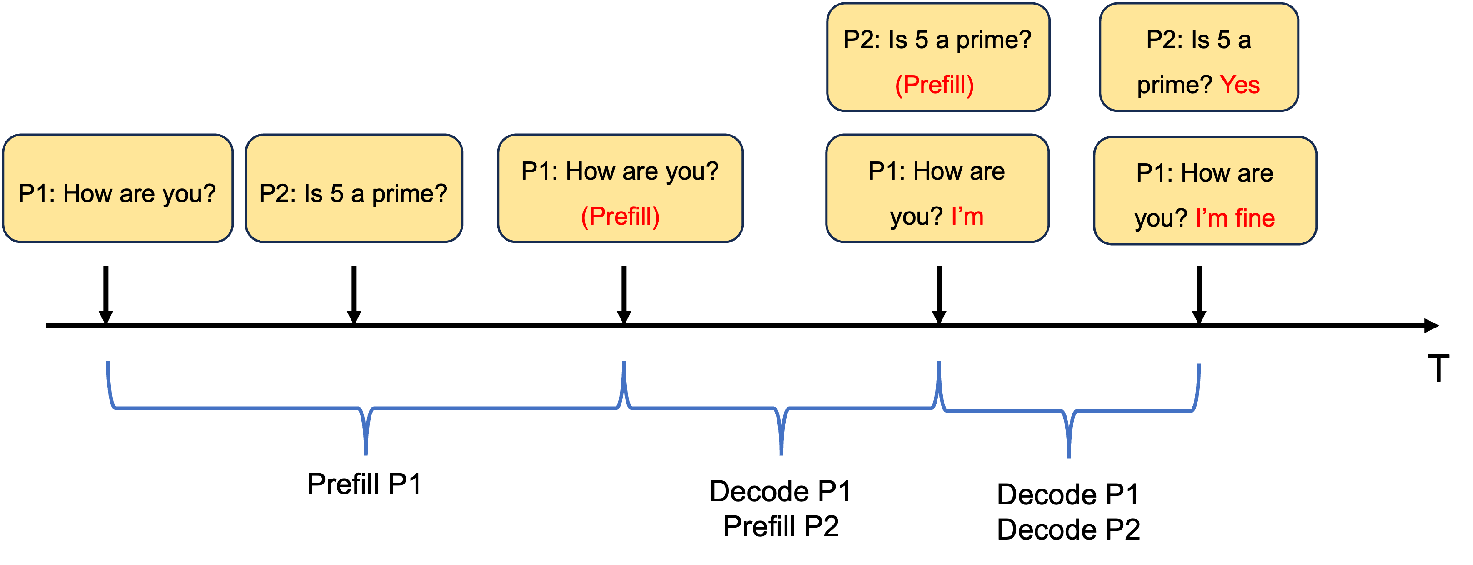
\includegraphics[width=0.55\linewidth]{Experiments_pdf/fig_batching1.pdf}
    \caption{Example of batching and scheduling with two prompts. The three GPU iterations shown are a prefill-only batch for \(P_1\), a mixed batch that decodes \(P_1\) while prefilling \(P_2\), and a decode-only batch for both prompts.}
    \label{fig:batching_example}
\end{figure}

We next specify the service time of an iteration. In Transformer inference, prefill evaluates the input sequence and creates the initial KV cache; thereafter, each decode iteration produces one token per active prompt while attending to the prompt's cached history. For a decode-dominated batch, the batch KV-cache size is therefore a natural workload descriptor. Let \(B^t\) denote the batch processed at iteration \(t\), let \(j(i)\) be the type of prompt \(i\), and let \(s_i^t\) be its current stage. A prefill prompt has \(s_i^t=0\) and initializes \(l_{j(i)}\) units of KV cache, while a decode prompt at stage \(s_i^t\) reads and extends a cache of size \(l_{j(i)}+s_i^t\). Guided by profiling studies of LLM serving workloads~\citep{agrawal2023sarathi,kwon2023efficient,zhong2024distserve}, we approximate iteration time by
\begin{equation}
\label{eq:time_consump}
    \tau(B^t) = d_0 + d_1 \sum_{i\in B^t} \bigl(l_{j(i)} + s_i^t\bigr),
\end{equation}
where \( d_0 \) is the fixed per-iteration overhead and \( d_1 \) is the marginal time cost per cached token. The affine form separates this fixed overhead from the marginal cost of serving larger KV caches. It captures the admission-control trade-off central to our model: admitting more prompts spreads \(d_0\) across more generated tokens and can therefore raise throughput, but it also lengthens subsequent iterations and consumes scarce GPU memory through larger KV caches. This regime is especially relevant because prompts typically spend most of their lifetime in decode, so admission decisions primarily determine the population and age distribution of active caches. Figure~\ref{fig:inference time} reports A100~80GB validation results for Llama-2-7B with the prompt setting fixed at input length \(256\) and output length \(20\). We vary the number of requests in the batch from \(1\) to \(256\) and record batch inference time across batch states in which the active requests may be at different decode stages. The horizontal axis is the total number of tokens stored in the KV cache across active requests, corresponding to \(\sum_{i\in B^t}(l_{j(i)}+s_i^t)\) for a serving iteration \(t\). Because the stages \(s_i^t\) vary across requests and iterations, batches with similar numbers of requests can have different total cached-token counts, producing the scattered validation points around the affine fit. Appendix~\ref{app:gpu_validation} reports additional simulator-validation and end-to-end GPU experiments for the same hardware setting.

The same formulation can accommodate other calibrated service-time curves. When prefill dominates, especially when prefill lengths are highly heterogeneous, input attention can add nonlinear length effects; mixed prefill-decode batches and hardware saturation can create distinct compute-bound and memory-bound regimes. These effects can be represented by replacing~\eqref{eq:time_consump} with a monotone function of batch composition, including piecewise-linear specifications such as \(\tau(b') = c + a\max\{0,b'-b_0\}\)~\citep{li2025throughput}. Prefill-decode disaggregated serving gives the complementary case: prefill work is routed to separate workers, and the decode server repeatedly executes one-token decode steps, making aggregate KV-cache usage an especially accurate state variable for iteration time~\citep{patel2024splitwise,zhong2024distserve}. Thus the affine model is both a close approximation in decode-centered settings and a transparent first-order primitive for the fluid analysis. It keeps the central operational trade-off explicit: larger batches improve utilization, but they also increase iteration time and memory pressure. Even when a richer calibrated service-time model is needed, the same perspective remains useful: the scheduler must control the population and decode-stage mix of resident prompts because these quantities determine both memory pressure and future service times.

\begin{figure}
    \centering
    
\includegraphics[width=0.55\linewidth]{Experiments_pdf/inference_time_comparison.pdf}
    \caption{Batch inference time of Llama-2-7B on a single NVIDIA A100~80GB GPU. We fix the prompt length at \(256\) tokens and the output length at \(20\) tokens, and vary the number of requests in the batch from \(1\) to \(256\). Each validation point corresponds to a batch state; requests in the same batch may be at different decode stages, so the horizontal axis reports the resulting total number of tokens stored in the KV cache across active requests. The vertical axis reports measured batch inference time. The affine fit indicates an approximately linear relationship between batch inference time and total cached tokens.}
    \label{fig:inference time}
\end{figure}

\subsection{Memory Constraint and Challenges}

The service-time model above describes how a batch uses the GPU in one iteration. The second constraint is intertemporal: a prompt that remains in service carries its KV cache across iterations, and this cache grows as decode progresses. Hence the scheduling state must track not only the current batch \(B^t\), but all prompts whose KV caches are currently resident on the GPU.

\textbf{Memory Constraint}: At all times \(t\), the total KV cache stored on the GPU must not exceed capacity \(C\):
\begin{equation}
\label{eq:memory_constraint}
\sum_{i \in \mathcal{G}^t} (l_{j(i)} + s^t_i) \le C,
\end{equation}
where \(\mathcal{G}^t\) is the set of prompts whose KV caches are resident on the GPU at time \(t\). This set includes the current batch \(B^t \subseteq \mathcal{G}^t\) as well as prompts that are waiting between iterations while retaining their KV caches on the GPU. Here \(j(i)\) is the type of prompt \(i\), and \(s_i^t \in \{0,1,\dots,l_{j(i)}'\}\) is its current decode progress. Prompts that have not yet been prefilled are not in \(\mathcal{G}^t\); once their KV cache is allocated, their memory contribution grows from \(l_{j(i)}\) with each generated token. If the constraint~\eqref{eq:memory_constraint} cannot be satisfied, the server must \textit{evict} resident prompts by discarding their KV caches. We model eviction as last-in-first-out: the most recently admitted prompts are evicted first until enough memory is freed. An evicted prompt loses its accumulated computation and restarts from prefill, re-entering the scheduling queue as a new job. This restart rule can create an eviction cascade: each eviction relieves memory pressure temporarily, but the restarted prompts return to the queue, raise future admission pressure, and can force additional evictions. The following example illustrates this mechanism.

\begin{example}[Dynamic Memory Growth and Eviction]
\label{ex:memory_growth}
Consider the running toy prompt ``Hello,'' which receives the one-token response ``Hi.'' This prompt type has prefill length \(l=1\) and decode length \(l'=1\). A prompt waiting for prefill uses no KV cache. Once its prefill is processed, the prompt becomes resident and uses one unit of KV cache; after it generates its single decode token, it uses \(l+1=2\) units just before completion. Suppose the GPU has capacity \(C=12\). One full-memory iteration can process four prefills and four decodes: the four newly prefilled prompts require \(4\times1=4\) units, and the four prompts already in decode require \(4\times2=8\) units, for a total of \(12\) units and four completions.

Now suppose three prompts are already decoding, using \(3\times2=6\) units, and the scheduler admits six new prompts for prefill, using another \(6\times1=6\) units during the iteration. After the iteration, the three old prompts complete and release their caches, while the six newly admitted prompts move into decode and now require \(6\times2=12\) units, filling memory. If four more prompts arrive next, admitting their prefills requires four additional units. The only way to create this space is to evict two resident decode prompts, each freeing two units. These evicted prompts lose their KV caches and return to the queue as new jobs, where they compete with subsequent arrivals and can force further evictions.

This example highlights the \textbf{eviction cascade} and the admission trade-off behind it. A larger batch can raise throughput because the fixed per-iteration overhead is shared across more generated tokens, but every admitted prompt also creates a KV cache that stays on the GPU and grows one token at a time until completion. If the scheduler admits too many prompts now, later decode iterations may leave too little memory for new arrivals, forcing eviction and restart. When output lengths are unknown, this decision must be made before the scheduler knows how long each prompt will remain in memory. Section~\ref{sec:fluid} formalizes the balanced admission level at which arrivals, completions, and memory growth can be kept in balance.
\end{example}

\subsection{Objective and Policy Space}

We evaluate a scheduling policy over a finite horizon \([0,T]\). The primary efficiency metric, denoted \(\throughput^{(T,\pi)}\), is \textit{effective throughput}: the average number of decode tokens from prompts that complete under policy \(\pi\). Tokens generated before a prompt is evicted do not count, because eviction discards the prompt's KV cache and returns it to prefill. This convention makes memory overflow part of the performance criterion rather than a separate implementation detail. For a fixed arrival process, effective throughput is capped by the offered decode-token load. A policy falls below this cap when it leaves capacity idle or admits work that later restarts instead of completing. Admission control must therefore balance utilization against memory feasibility: admitting enough prompts to exploit the GPU, but not so many that KV-cache growth forces eviction. Maintaining this balance over a wider range of arrival rates expands the realized stability region, and under overload it keeps completed work close to the server's usable capacity. We also evaluate \(\Latency^{(T,\pi)}\), the average elapsed time from prompt arrival to completion, and \(\TTFT^{(T,\pi)}\), the average elapsed time from arrival to the first generated output token. These delay metrics capture service quality beyond aggregate output. In particular, TTFT rules out policies that keep completion counts high by repeatedly prioritizing short prompts while delaying the first service of longer prompts. Later sections introduce the fluid model and use it to establish throughput, latency, and TTFT guarantees for the proposed policies.

Let \(\Pi\) denote the class of admissible online policies. At each decision epoch \(t\), a policy \(\pi \in \Pi\) observes the prompts that have arrived, their input lengths, their current stages \(s_i^t\), and whether their KV caches are resident on the GPU. The policy is non-anticipating: it cannot use future arrivals or a prompt's output length before that length is revealed by completion.

Given this information, the policy chooses which waiting prompts to admit, which resident prompts to batch in the current iteration, and whether to preempt or evict prompts. Preemption pauses a resident prompt while keeping its KV cache on the GPU, so it can resume without recomputation. Eviction removes the KV cache to free memory; under the LIFO rule used here, the most recently admitted resident prompts are evicted first, and each evicted prompt returns to stage \(s=0\) and must restart from prefill. All decisions must satisfy the memory constraint~\eqref{eq:memory_constraint} after the resulting state transition.
% This formulation
% encapsulates the potential trade-offs between resource efficiency and service quality: without the latency and TTFT constraints, the algorithm may always prioritize the shortest jobs in order to maximize the throughput and the latency of the long jobs can be very large in overloaded systems.

% \subsection{Unique Challenges and Comparison to Prior Work}

% This model poses distinct analytical and operational challenges not addressed by conventional scheduling literature:
% \begin{enumerate}
%     \item \textbf{Dynamic memory growth}: Unlike traditional jobs, prompts exhibit progressively increasing memory usage during decoding, complicating classical static memory allocation methods.
%     \item \textbf{Output length uncertainty}: Unlike Jaillet et al. (2025), which assumes known output lengths, our scenario reflects realistic settings where output predictions are unreliable, thus complicating analysis and batch formation strategies.
%     \item \textbf{Multi-stage process}: Prefill and decode phases differ significantly in computational patterns, necessitating a fluid approximation approach to handle their differing resource demands analytically.
% \end{enumerate}

% To address these challenges, we propose a fluid-based analytical framework and threshold-based policies (Sections~\ref{sec:fluid}-\ref{sec:nested_wait}) explicitly designed to operate efficiently under realistic conditions of output uncertainty and stochastic arrivals. This distinguishes our work analytically and practically from existing literature.
